\section{Résultats}

\paragraph*{Rendement théorique}
L'estimation de la température \(T_2\) est possible en regardant la couleur du fil chauffant. Celui-ci est observé comme étant rouge-orange ce qui correspond à une température (\(T_2 = 1143 \pm 70\)) \si{\kelvin} \cite{temp-fil}. Ainsi à l'aide de l'\autoref{eq:rend-theorie} et de la mesure de (\(T_1 = 295.0 \pm 0.1\)) \si{\kelvin} il est possible de calculer que (\(\eta_{theorie} = 74 \pm2\))\%.

\paragraph*{Rendement expérimental}
La puissance et le rendement expérimental du moteur de Stirling à été calculé en utilisant trois méthodes différentes. En utilisant la \autoref{fig:diag_pv} en \autoref{sec:image}, il est possible d'obtenir l'aire sous la courbe de \(A = (106 \pm 6)\) \si{\centi\meter\squared}. La calibration des axes avec \(V_\textrm{min} = (100 \pm 30)\) \si{\centi\meter\cubed}, \(V_\textrm{max} = (372 \pm 76)\) \si{\centi\meter\cubed}, \(p_\textrm{min} = (0.1 \pm 0.1)\) \si{\bar} et \(p_\textrm{max} = (0.55 \pm 0.05)\) \si{\bar} permet de trouver le travail \(W\). La mesure de la vitesse de rotation du volant d'inertie \(\omega = (24 \pm 1)\) \si{\radian\per\second} permet d'obtenir avec l'\autoref{eq:efficacite} et l'\autoref{eq:pm_pv} la puissance et le rendement.

La mesure de la force sur le disque de freinage de rayon \(R = (40.0 \pm 0.1)\) \si{\milli\meter} ainsi que la vitesse de rotation du volant d'inertie pour une distance donnée entre le disque et le volant permet d'obtenir à l'aide de l'\autoref{eq:pm_frein} la puissance, en supposant que \(\cos{\alpha} \approx 1\) puisque \(\alpha\), l'angle entre l'horizontale et l'aimant, restait proche de 0.

Enfin, la méthode de différence des flux permet de trouver avec l'\autoref{eq:pm_chaleur}, \(U = (13.41 \pm 0.05)\) \si{\volt}, \(I = (12.82 \pm 0.05)\) \si{\ampere} et \(\Delta T = (3.9 \pm 1)\) \si{\kelvin}, une autre puissance et efficacité. Tous les résultats sont reportés dans le \autoref{tab:pm_efficacite}.

\begin{table}[h]
    \centering
    \begin{tabulary}{\linewidth}{C C C C C}
        \toprule
        Méthode & Diagramme PV & Frein (min) & Frein (max) & Différence des flux \\
        \midrule
        \(P_m\) [\si{\watt}] & \(11 \pm 5\) & \(0.50 \pm 0.05\) & \(1.41 \pm 0.08\) & \(96 \pm 3\) \\
        \(\eta\) & (\((6 \pm 3)\))\% & \(0.10 \pm 0.03\)\% & \((0.82 \pm 0.05)\)\% & \((56 \pm 1)\)\% \\
        \bottomrule
    \end{tabulary}
    \caption{Puissances et rendements calculés avec les trois méthodes}
    \label{tab:pm_efficacite}
\end{table}

\paragraph*{Caractéristiques couple-régime et rendement-régime}
Les mesures prises en éloignant le disque de freinage de l'arbre de rotation permettent d'obtenir les diagrammes reliant la vitesse angulaire au couple en \autoref{fig:couple-regime} et au rendement en \autoref{fig:rend-regime}. Le couple a été calculé par l'\autoref{eq:couple} et le rendement à l'aide des \autoref{eq:efficacite} et \autoref{eq:pm_frein}.

\begin{figure}[h]
    \centering
    \begin{subfigure}{0.5\linewidth}
        \centering
        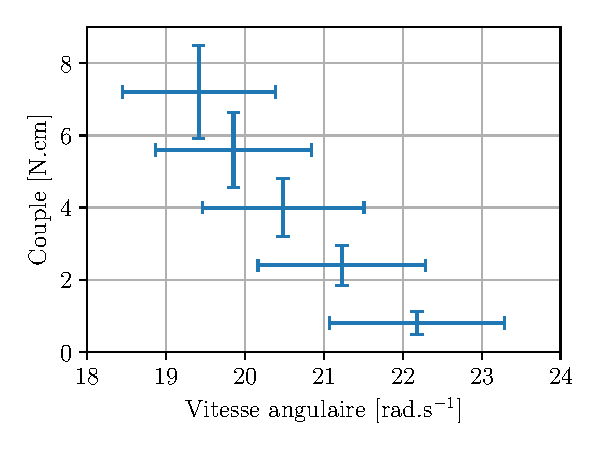
\includegraphics[width=\linewidth]{figures/couple-regime.pdf}
        \caption{}
        \label{fig:couple-regime}
    \end{subfigure}%
    \begin{subfigure}{0.5\linewidth}
        \centering
        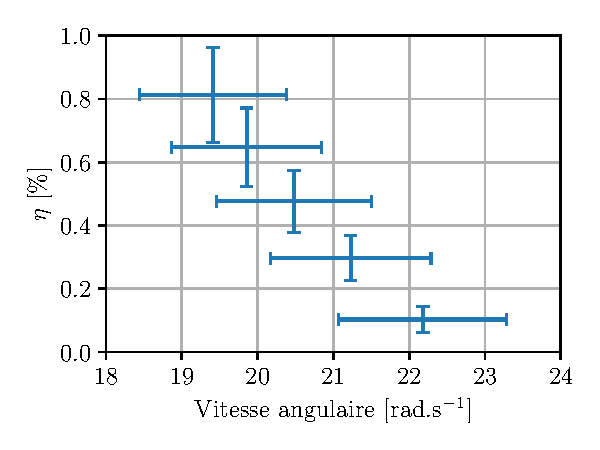
\includegraphics[width=\linewidth]{figures/rendement-regime.pdf}
        \caption{}
        \label{fig:rend-regime}
    \end{subfigure}
    \caption{Diagrammes (a) couple-régime et (b) rendement-régime}
\end{figure}



\begin{minipage}{\linewidth}
    \begin{wrapfigure}{R}{0.5\linewidth}
        \centering
        \vspace{-1.4cm}
        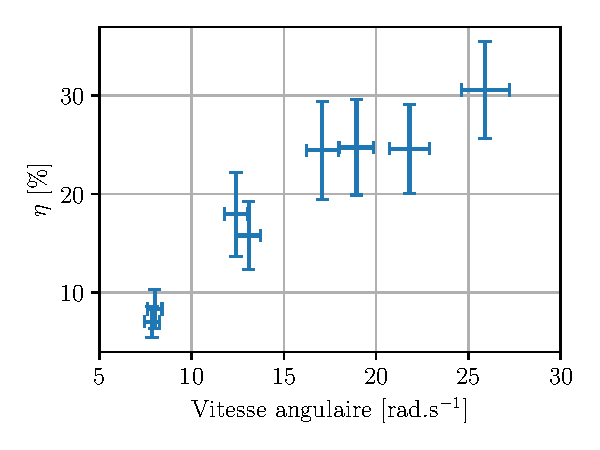
\includegraphics[width=\linewidth]{figures/rend-frigo.pdf}
        \caption{Rendement du cycle frigorifique en fonction du régime de l'arbre de rotation}
        \label{fig:rend-frigo}
    \end{wrapfigure}

    \paragraph*{Rendement du cycle frigorifique}
    Les mesures des puissances fournies au moteur et au filament de compensation permettent un calcul du rendement par l'\autoref{eq:rend-frigo}. La valeur de la température d'équilibre du système entre le refroidissement et la compensation n'a pas été exactement constante sur l'ensemble des mesures mais a tout de même variée de moins de 10 \si{\kelvin}. Les rendements obtenus sont représentés avec leurs barres d'erreur sur la vitesse angulaire et sur le rendement en \autoref{fig:rend-frigo}.
\end{minipage}


